

\begin{juliacode}
using Plots
pyplot()
x = linspace(0, 2*pi)
println(x)

\end{juliacode}
\begin{juliaout}
linspace(0.0,6.283185307179586,50)
\end{juliaout}

\begin{juliacode}
p = plot(x, sin(x), size =(900,300))
\end{juliacode}




\begin{juliaterm}
julia> plot(x, sin(x))

\end{juliaterm}
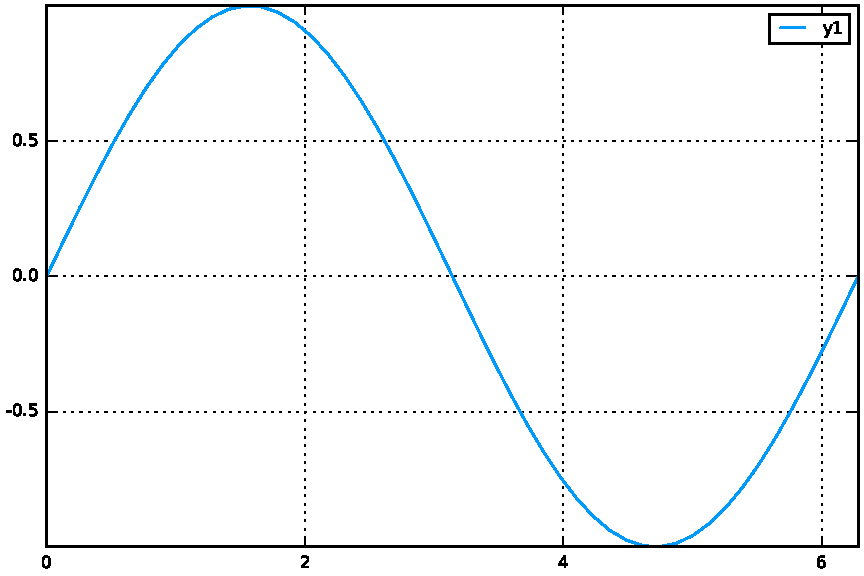
\includegraphics[width=\linewidth]{figures/plotsjl_test_2_1.pdf}



\begin{juliacode}
plot(rand(100) / 3,reg=true,fill=(0,:green))
scatter!(rand(100),markersize=6,c=:orange)
\end{juliacode}
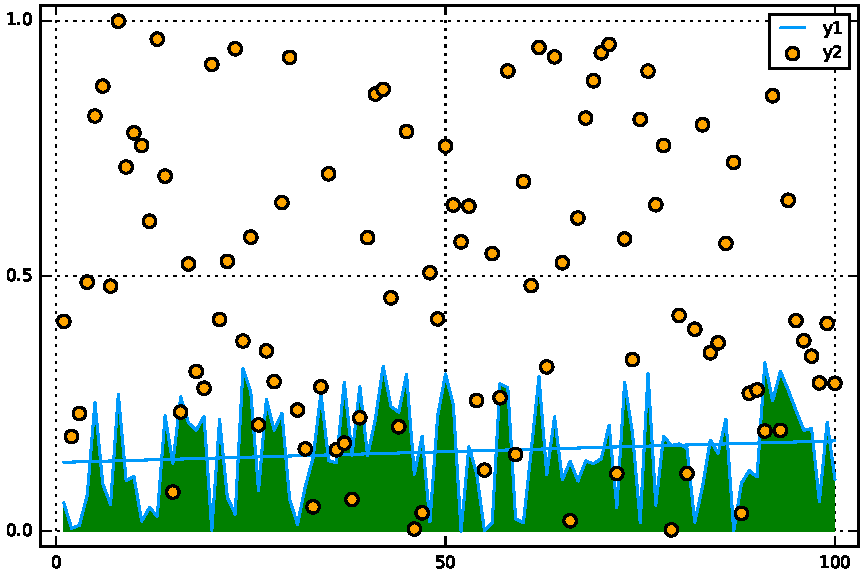
\includegraphics[width=\linewidth]{figures/plotsjl_test_3_1.pdf}



\begin{juliaterm}
julia> plot(rand(100) / 3,reg=true,fill=(0,:green))


\end{juliaterm}
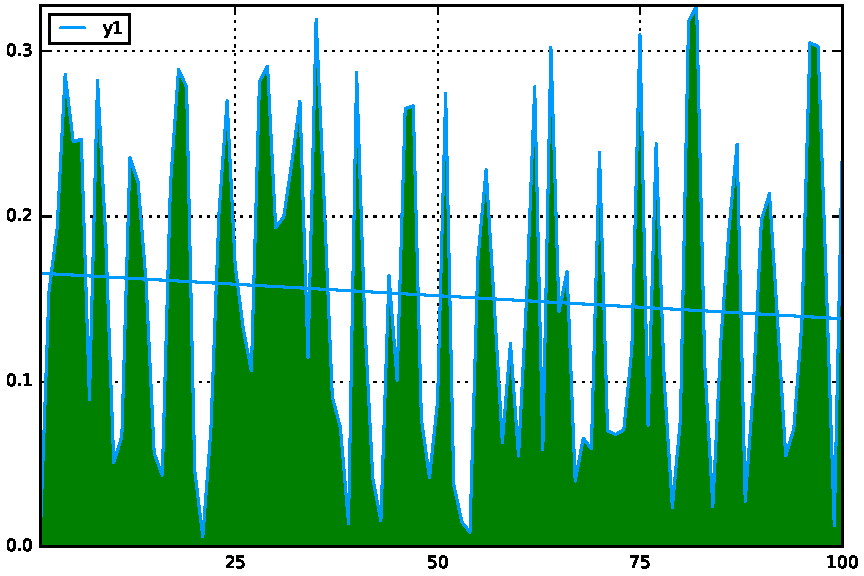
\includegraphics[width=\linewidth]{figures/plotsjl_test_4_1.pdf}

\begin{juliaterm}
julia> scatter!(rand(100),markersize=6,c=:orange)

\end{juliaterm}
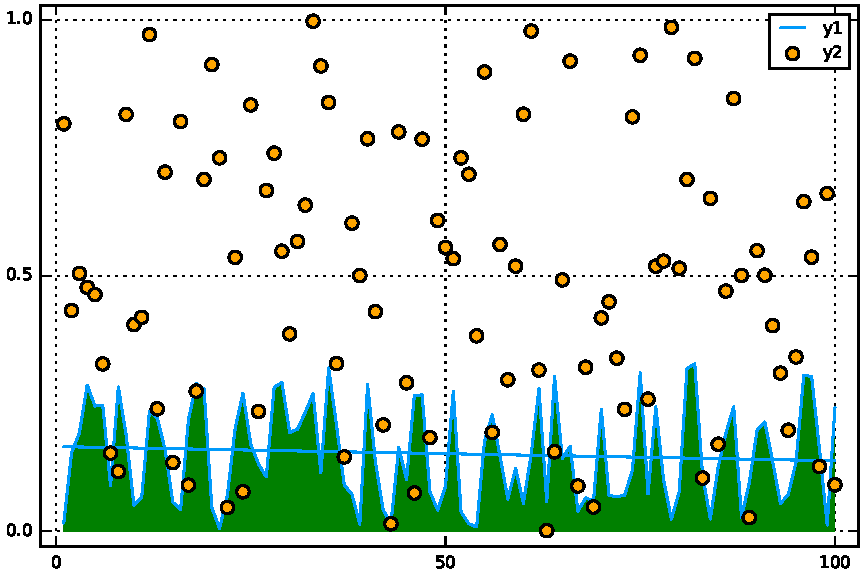
\includegraphics[width=\linewidth]{figures/plotsjl_test_4_2.pdf}




\begin{figure}[htpb]
\center
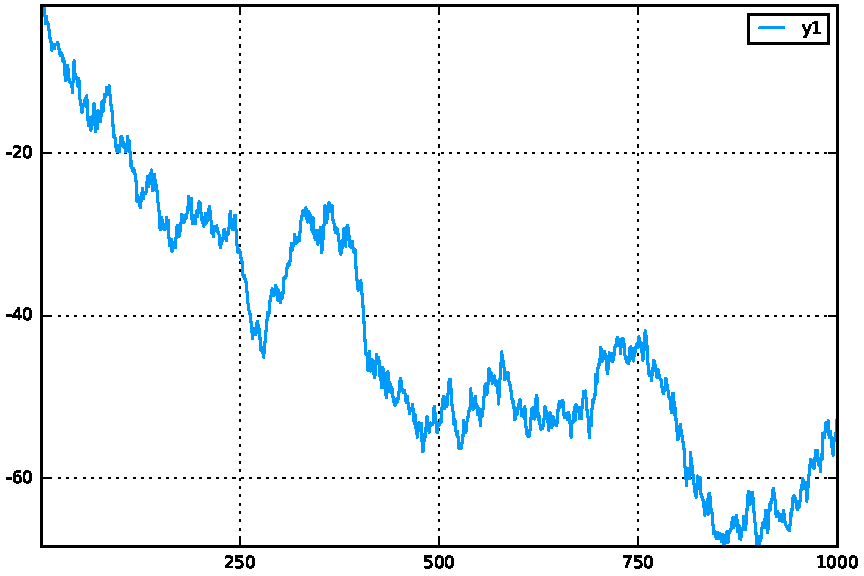
\includegraphics[width=\linewidth]{figures/plotsjl_test_random_1.pdf}
\caption{A random walk.}
\label{fig:random}
\end{figure}
